%%============
%%  ** Author: Shepherd Qirong
%%  ** Date: 2021-12-11 17:07:45
%%  ** Github: https://github.com/ShepherdQR
%%  ** LastEditors: Shepherd Qirong
%%  ** LastEditTime: 2021-12-19 14:34:25
%%  ** Copyright (c) 2019--20xx Shepherd Qirong. All rights reserved.
%%============



\documentclass[UTF8]{article}
\usepackage{ctex}
\usepackage{amsmath,amsthm,amsfonts,amssymb,bm,mathrsfs,upgreek} 
\usepackage{graphicx}
\usepackage[paper=a4paper,top=3.5cm,bottom=2.5cm,
left=2.7cm,right=2.7cm,
headheight=1.0cm,footskip=0.7cm]{geometry}
\usepackage{color}
\usepackage{multirow,booktabs}

\RequirePackage{setspace}%%linespace
\setstretch{1.523}


\begin{document}
\section{Introduction}
Today is 20211211, and I deciede to note down all of my knowledge about problems in this notebook. Actually we think for a while whether to seperatre the knowledge into different documents.

\section{Physics}

\subsection{Energy}

\subsubsection{T0001}
The coordinate of free fall ball ends. With energy equation, we have $GH = \mu G \xi kH$, considering of the backward length, we draw the figure and it can be transfered from the figure $y = |x|$. We have the coordinate
at $[1-\vert (\mu k)^{-1} \pmod 2 -1 \vert ]kH $.
\begin{figure*}[h]
    \centering
    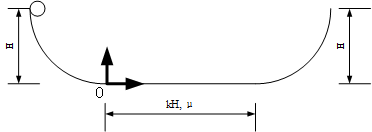
\includegraphics[width=0.5\textwidth]{../../resources/T0001.png}
    \caption{[T0001: Where the ball ends]}
    \label{fig:1}
\end{figure*}

\subsubsection{T0002}
Suppose the ball free falls tangently into a circle, at the top of the circle, to matian the circular movement, $mg + F_{support} = mv^2/R$, since $m(n-2)gR = 1/2mv^2$, we have $F_{support} = mg(2n-5)$.

When $n<=1$, it is easy to see that the ball swings. When $n>=2.5$, the ball keeps going along the circle. When $n \in (1,2.5)$, suppose the ball is at the angle $\theta$ as shown in the figure, the energy equation shows that $(nR-R + R \cos \theta) mg = 1/2 mv^2$, force equation shows that $F_{support} - mg \cos \theta = m v^2/R = 2mg(n-1+\cos \theta )$, so $F_{support}  = mg(2n-2+ 3\cos \theta )$. when $F_{support}  = 0$, the ball falls, and it falls at the angle $ \cos \theta = \frac{2}{3}(1-n)$.
\begin{figure*}[h]
    \centering
    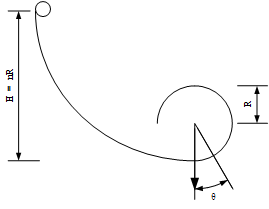
\includegraphics[width=0.5\textwidth]{../../resources/T0002.png}
    \caption{[T0002: Where the ball falls]}
    \label{fig:2}
\end{figure*}

\subsubsection{T0003}
When an object seperates into several parts, the velocity of each component is different. Using the momentum equation, we have $mv = (-dm)u+(v+dv)(m+dm)$, and we let $u = v+dv-v_{rel}$, so we have $0 = v_{rel} dm + m dv$, so $dv = -v{rel} \frac{dm}{m}$, the formula is integrated as $v_{final} - v_{0} = v_{rel} \ln \frac{m_0}{m_{final}}$. This means that when the rocket accolerates like this, the final mass needs to be quite small, because the logarithm function decreases rapidly, also the $v_{rel}$ needs to be big.

\begin{figure*}[h]
    \centering
    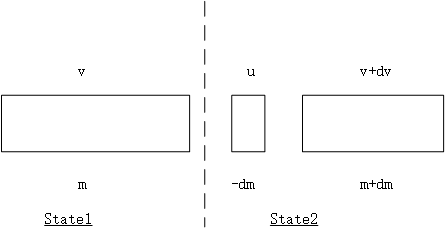
\includegraphics[width=0.5\textwidth]{../../resources/T0003.png}
    \caption{[T0003: Where the ball falls]}
    \label{fig:3}
\end{figure*}



\subsubsection{T0004}
AF=AE, AB=AC, AB=8. \\
1) BF = 2, DQ? \\
2) Prove $\sqrt 2AC - 2 AQ = BG$\\
3)The right figure, AE=AF=4, the little isosceles triangle rotates, use the middle point M construct another isosceles triangle, when $\min RN$, MR?\\
Solution:\\
1)We know how to simplify $\tan {(\alpha + \beta)}$, it is easy in $\bigtriangleup ADQ$, $DQ = \frac{8}{\sqrt2} \cdot \frac{1}{1+3}= \frac{4\sqrt 2}{7}$.\\
2) The formula is the same as $BG=2QD$, let $BF:=\delta, \angle CBE = \alpha$, we use triangles $\bigtriangleup BPF$ and  $\bigtriangleup BPG$ to get $BG = \frac{\delta \cos(\frac{\pi}{4}-\alpha)}{\cos \alpha}$ ,since$DQ = BD\tan \alpha$, and with the law of sines, we have 

\begin{equation}
    %\begin{split}
 \frac{BG}{DQ} = \frac{\delta}{BD} \cdot \frac{\cos(\frac{\pi}{4}-\alpha)}{\sin \alpha} = 2 \cdot \frac{\sin \alpha}{\sin(\frac{7\pi}{4}-\alpha)}\frac{\cos(\frac{\pi}{4}-\alpha)}{\sin \alpha} =2. \square 
%\end{split}
\end{equation}
3) the point M is on the circle with radius $r = 2\sqrt 2$, we establish the coordinate system with original point at the center of the circle. M is noted as $[x,y]^T$, point B is  $[-2r, -2r]^T$, M rotates along B to get N, 

\begin{equation}
    \begin{bmatrix}
        0 &1\\
        -1 & 0
    \end{bmatrix}
    \cdot     
    \begin{bmatrix}
        x+2r\\
        y+2r
    \end{bmatrix}
    + 
    \begin{bmatrix}
        -2r\\
        -2r
    \end{bmatrix}
    = 
    \begin{bmatrix}
        y\\
        -x-4r
    \end{bmatrix}
\end{equation}
so point R is $[y,-2r]^T$, $\min (x+2r)^2 \Rightarrow [x,y]^T = [-r,0]^T$, so $MR = \sqrt{(x-y)^2 + (y+2r)^2} = 2\sqrt {10}$.

\begin{figure*}[h]
    \centering
    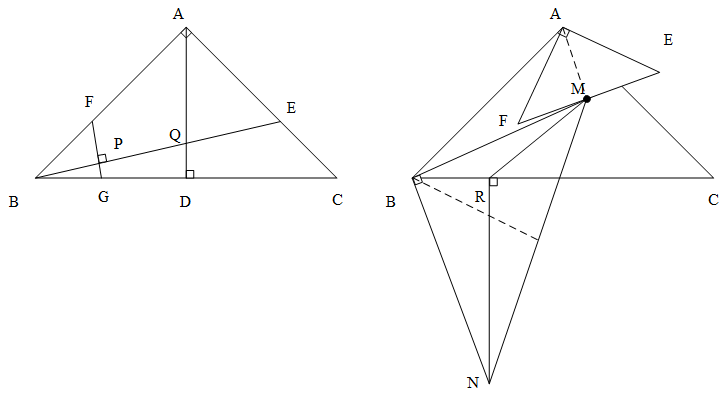
\includegraphics[width=0.5\textwidth]{../../resources/T0005_20211219_HigniorSchoolGeometry.png}
    \caption{[T0004:HigniorSchoolGeometry]}
    \label{fig:4}
\end{figure*}



\end{document}